\newcommand{\FigICEDUSTOverview}{
\begin{figure}[t]
\centering
%\fbox{
\includegraphics[width=1.00\textwidth,trim=0.85cm 0.5cm 0.5cm 0.5cm,clip=true]{figs/software/ICEDUST_structure}
%}
\caption{
Overview diagram for the ICEDUST framework.
Data produced from simulation or taken in the real experiment are treated identically through the calibration and onwards up to analysis.
}
\figlabel{software:ICEDUSTOverview}
\end{figure}
}

\newcommand{\FigNDTwoEighty}{
\begin{figure}[t]
\centering
\includegraphics[width=0.95\textwidth]{figs/software/ND280SoftwareDiagram}
\caption{
Overview diagram for the ND280 framework.
}
\figlabel{software:ND280}
\end{figure}
}

\newcommand{\FigSimulationOverview}{
\begin{figure}[t]
\centering
%\fbox{
\includegraphics[width=1.00\textwidth]{figs/software/Simulation_structure}
%}
\caption{
Diagram showing the stages used to simulate COMET.
The timing schematics on the right show how a simulated event is built up, firstly by producing many individual proton interactions with the production target,
then by transporting the secondary particles to produce energy deposits in the detector, which are then combined with the truth hits from other proton events to produce a realistic bunch structure.
Finally these bunch events are processed through the detector response simulation to produce fake waveforms and other detector read-outs.
}
\figlabel{software:SimulationOverview}
\end{figure}
}

\newcommand{\FigGeometryHeirarchy}{
\begin{figure}[t]
\centering
%\fbox{
\includegraphics[width=0.70\textwidth]{figs/software/ComponentHeirarchy}
%}
\caption{
How parameters are shared amongst different components.
The Controller of component 1.a in red has access to the parameters managed by Controllers of components contained in the larger violet region.
}
\figlabel{software:componentHeirarchy}
\end{figure}
}

\newcommand{\FigGeometryParameters}{
\begin{figure}[t]
\lstinputlisting[style=customc]{figs/software/demo-parameters.mac}
\caption{
An example set of parameters definitions which control the building of the Torus2 geometry.
}
\figlabel{software:geom:paramAssignments}
\end{figure}
}

\newcommand{\FigPiYieldHadronCodes}{
\begin{figure}[b]
\centering
%\fbox{
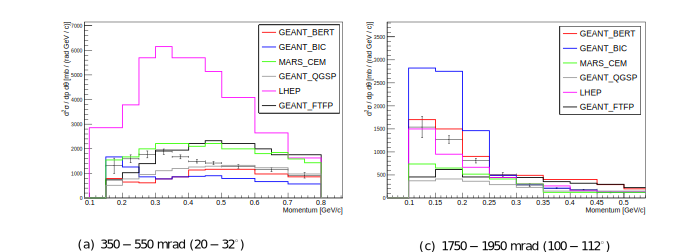
\includegraphics[width=0.95\textwidth,trim=2cm 1cm 0.8cm 0.5cm,clip=true]{figs/software/PionYield_AEdmondsThesis}
%}
\caption{
Comparison of various hadron production codes with experimental data from the HARP experiment from the thesis of A. Edmonds~\cite{AEdmondsThesis}.
Points with error bars are the experimental data.  Left: double differential-production cross section for pion production from 20 to 32\degree with respect to the incoming proton direction, right: from 100 to 112\degree.
The hadron production code that best reproduces the data depends strongly on which angular region one looks at.
}
\figlabel{software:piYield}
\end{figure}
}

\newcommand{\FigSimulationPhysicsClasses}{
\begin{figure}[tb]
\centering
%\fbox{
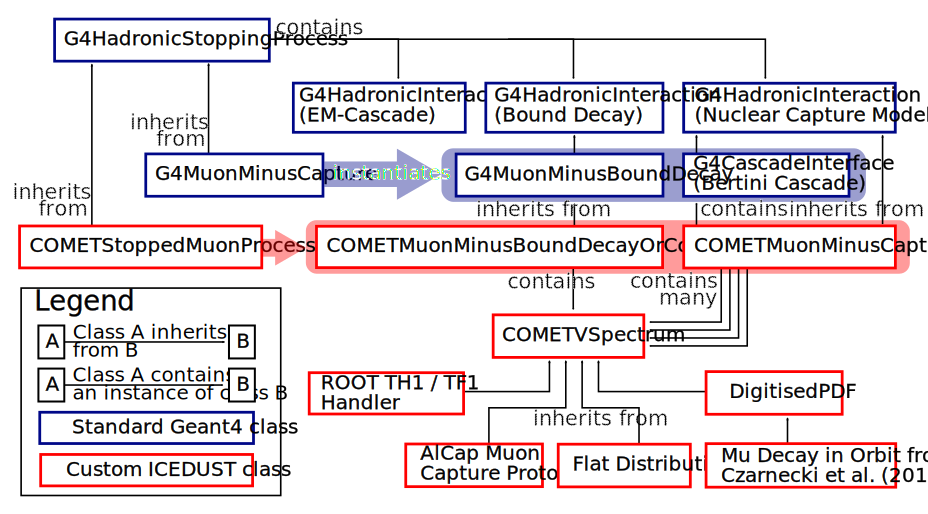
\includegraphics[width=1.00\textwidth]{figs/software/SimulationMuonPhysicsClasses}
%}
\caption{
The various classes involved in simulating the various processes of stopped negative muons.
%Classes in red have been implemented for COMET and augment the existing Geant4 classes which are shown in blue.
The standard Geant4 model is activated by registering `G4MuonMinusCapture' which instantiates `G4MuonMinusBoundDecay' and `G4CascadeInterface' to run the \ac{DIO} and nuclear capture respectively.
To use the custom COMET muon physics, an instance of `COMETStoppedMuonProcess' should be registered which sets up `COMETMuonMinusBoundDecayOrConversion' to produce the electron (and possibly neutrinos) from \ac{DIO} or conversion, and `COMETMuonMinusCapture' to do the nuclear capture.
}
\figlabel{software:ExtendedMuonClasses}
\end{figure}
}

